\graphicspath{ {Figures/implementation/} }
\chapter{Υλοποίηση}\label{ch:Implementation}
\section{Back-End}
	\subsection{Parse}
	\subsection{NodeJS}
		
\section{Front-End Cloud App}
	\subsection{JS}
	\subsection{jQuery και AngularJS}
	\subsection{Screenshots}
	\subsection{Social Networking Integration}
	\subsection{Testing and Tools}
		\subsubsection{Unit Testing}
		\subsubsection{Infrastucture Testing}
		\subsubsection{Performance Testing}
		\subsubsection{Browser Compatibility Testing}

\section{Android}
	\subsection{Activities}
	\subsection{Screenshots}
	\subsection{Social Networking Integration}
	\subsection{Testing and Tools}
	Στο παρόν κεφάλαιο θα αναφερθούμε αρχικά στο περιβάλλον ελέγχου που μας παρέχει το Android καθώς και στους διαφορετικού τύπους ελέγχου που μπορούμε να εκτελέσουμε. Στην συνέχεια θα αναφερθούμε στους ελέγχους που πραγματοποιήσαμε καθώς και στα αποτελέσματα τους.
	
	Η δυνατότητα αυτοματοποιημένου έλεγχου των εφαρμογών του λειτουργικού Android είναι ιδιαίτερα σημαντική λόγω του μεγάλου αριθμού διαφορετικών συσκευών που υπάρχουν στην αγορά. Λόγω αυτού είναι αδύνατον να δοκιμάσουμε μία εφαρμογή με όλες τις δυνατές ρυθμίσεις μιας συσκευής, για αυτό αποτελεί συνηθισμένη πρακτική η εκτέλεση δοκιμών με τις πιο συνηθισμένες ρυθμίσεις. Στόχος είναι η επίτευξη ενός υψηλού ποσοστού κάλυψης δοκιμών (test coverage), έτσι ώστε να παράγουμε μια εφαρμογή απαλλαγμένη από σημαντικά σφάλματα αλλά και να διευκολύνουμε την συντήρηση και επέκτασή της στο μέλλον.
	
	Οι δοκιμές στο λειτουργικό σύστημα Android βασίζονται στο JUnit, και μπορούν να χωριστούν σε δύο μεγάλες κατηγορίες όπως φαίνεται στο σχήμα \ref{fig:categories_of_android_tests} ανάλογα με το αν απαιτούν το λειτουργικό συστήματα android ή αν χρειάζονται μόνο την εικονική μηχανή της Java (JVM - Java Virtual Machine) κατά την διάρκεια της εκτέλεσής τους\cite{androidTesting}.
	
	\begin{figure}[h]
	    \centering
	    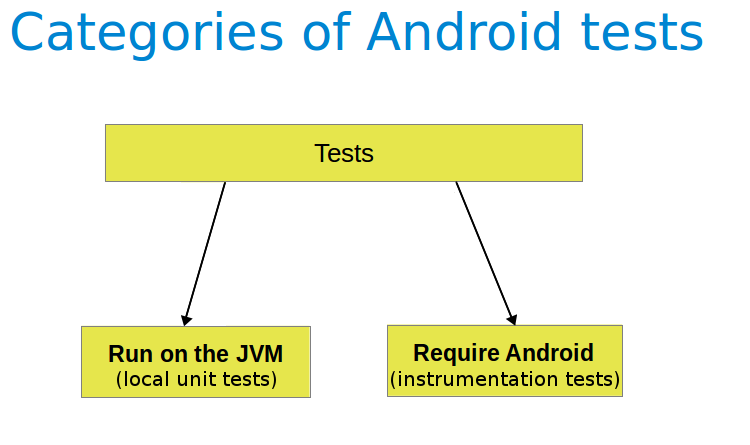
\includegraphics[width=0.7\textwidth]{categories_of_android_tests.png}
	    \caption{ Κατηγορίες δοκιμών στο Android}
	    \label{fig:categories_of_android_tests}
	\end{figure}
	
	Εφόσον είναι εφικτό, είναι πάντα προτιμότερο να τρέχουμε τις δοκιμές στην εικονική μηχανή της Java, δεδομένου ότι απαιτεί πολύ λιγότερο χρόνο σε σχέση με το χρόνο που απαιτείται για την εγκατάσταση και εκτέλεση της εφαρμογής σε μία συσκευή Android. Στην συνέχεια της παρούσας ενότητας η εφαρμογή που δοκιμάζεται θα αποκαλείται \textit{εφαρμογή υπό δοκιμή}.
		\subsubsection{Unit Testing (Δοκιμή μονάδας)}
		Έλεγχοι τύπου unit testing χρησιμοποιούνται για την δοκιμή μικρών μεμονωμένων στοιχείων της εφαρμογής, χωρίς να εξετάζεται η αλληλεπίδραση τους με άλλα στοιχεία της εφαρμογής. Δηλαδή όπως δηλώνει και το όνομα τους, εξετάζουν τη συμπεριφορά ενός στοιχείου ως ξεχωριστή μονάδα. Για να γίνει καλύτερα αντιληπτό το παραπάνω, ας υποθέσουμε ότι θέλουμε να δοκιμάσουμε ένα κουμπί το οποίο αναμένουμε να μας μεταφέρει σε μια άλλη οθόνη.  Στα πλαίσια της δοκιμής μονάδας θα γίνει έλεγχος αν η πρόθεση (intent) για αλλαγή οθόνης δημιουργήθηκε σωστά και όχι αν μεταφερθήκαμε στην άλλη οθόνη. Σε περίπτωση όμως που εκτελούσαμε δοκιμές ενσωμάτωσης (instrumentation testing βλ. ενότητα \ref{sssec:instrumentation_testing}) θα έπρεπε να γίνει έλεγχος ότι η επόμενη οθόνη ξεκίνησε όπως αναμέναμε.
		
		Τα Unit tests χρησιμοποιούν το JUnit test framework και δεν πρέπει να χρησιμοποιούν λειτουργίες από το Android API έτσι ώστε να είναι σε θέση να τρέξουν στην εικονική μηχανή της Java (JVM) κάτι το οποίο απαιτεί πολύ λιγότερο χρόνο σε σχέση με το αν χρειαζόντουσαν να τρέξουν σε περιβάλλον Android. Κάθε εξάρτηση από το λειτουργικό Android θα πρέπει να αντικατασταθεί στον κώδικα που θέλουμε να δοκιμάσουμε με κάποιο mocking framework όπως είναι το Mockito. 
		
		Παρακάτω βλέπουμε ένα απλό JUnit test που φτιάξαμε με σκοπό να δοκιμάσουμε την λειτουργία της συνάρτησης που ελέγχει την εγκυρότητα του κωδικού χρήστη.
		\lstinputlisting[language=Java]{ValidatorTest.java}  
		\subsubsection{Instrumentation Testing}\label{sssec:instrumentation_testing}
		Όταν θέλουμε να δοκιμάσουμε κλάσεις και λειτουργίες της εφαρμογής οι οποίες αλληλεπιδρούν με το λειτουργικό Android τότε δημιουργούμε τις λεγόμενες δοκιμές ενσωμάτωσης (instrumentation tests). Το Android API για δοκιμές παρέχει στον προγραμματιστή άγκιστρα (hooks) μέσω των οποίων μπορεί να αλληλεπιδράσει με τον κύκλο ζωής των στοιχείων λογισμικού και της εφαρμογής. Αυτά τα άγκιστρα απαρτίζουν το instrumentation API και επιτρέπουν στις δοκιμές να ελέγχουν γεγονότα από τον κύκλο ζωής (life cycle events) και την αλληλεπίδραση του χρήστη.

		Υπό κανονικές συνθήκες ένα στοιχείο του Android ακολουθεί έναν κύκλο ζωής που έχει καθοριστεί από το σύστημα βάση της αλληλεπίδρασης του με τον χρήστη. Για παράδειγμα, όταν δημιουργείται μια πρόθεση (intent) για έναρξη κάποιου Activity, καλείται η μέθοδος onCreate() του εν λόγω Activity. Στην συνέχεια αν ο χρήστης ανοίξει κάποια άλλη εφαρμογή, καλείται η μέθοδος onDestroy() του Activity . Το instrumentation API αν και δεν επιτρέπει στον προγραμματιστή να καλέσει αυτές τις μεθόδους απευθείας, του επιτρέπει να εξομοιώσει πλήρως την συμπεριφορά ενός χρήστη η οποία προκαλεί τέτοια γεγονότα. Για παράδειγμα επιτρέπει στον προγραμματιστή να στείλει γεγονότα πλήκτρων ή αφής, έλεγχοντας με αυτό τον τρόπο το κύκλο ζωής της υπό δοκιμής εφαρμογής\cite{androidTestingBook}.

		Τα instrumentation tests δεν γίνεται να τρέξουν στο JVM αλλά χρειάζονται περιβάλλον με λειτουργικό σύστημα Android. Μπορούν να τρέξουν είτε σε πραγματική συσκευή Android η οποία έχει συνδεθεί με τον υπολογιστή στον οποίο γίνεται η ανάπτυξη, είτε σε εικονική συσκευή Android. Δεδομένου του πλήθους των συσκευών που τρέχουν το λειτουργικό σύστημα Android, και συνυπολογίζοντας τις διάφορες εκδόσεις που μπορεί να τρέχει κάθε συσκευή, κάθε δοκιμή θα πρέπει να γίνεται με χρήση εξομοίωσης σε διάφορα επίπεδα API αλλά και μεγέθη οθονών. Για παράδειγμα αν η εφαρμογή υποστηρίζει επίπεδο API μεγαλύτερο του 14 θα πρέπει να γίνει έλεγχος για κάθε API μεγαλύτερο του 14 με τουλάχιστον 2 διαφορετικά μεγέθη οθόνης για κάθε API. 
		
		Όπως γίνεται εμφανές από τα παραπάνω το τρέξιμο των instrumentation tests αποτελεί μια ιδιαίτερα χρονοβόρα διαδικασία. Για την εξομάλυνση αυτού του προβλήματος υπάρχουν υπηρεσίες μέσω των οποίων οι δοκιμές μπορούν να γίνουν στο υπολογιστικό νέφος. Παρακάτω βλέπουμε ένα παράδειγμα δοκιμών instrumentation που φτιάξαμε για να ελέγξουμε την λειτουργία επαναφοράς κωδικού.
		\lstinputlisting[language=Java]{ResetPassword.java}
		\subsubsection{Performance Testing}
		\subsubsection{Android API Level compatibility testing}

